\begin{figure}[htbp]
\centering
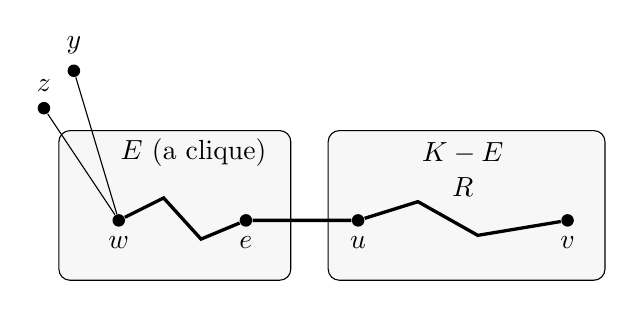
\begin{tikzpicture}[scale=.95,vertex/.style={circle,fill=black,inner sep=1.6pt}]
\draw[rounded corners,fill=black!3] (-.8,-.8) rectangle (2.3,1.2);
\node at (1,.9) {$E$ (a clique)};
\node[vertex,label=below:$w$] (w) at (0,0) {};
\node[vertex,label=below:$e$] (e) at (1.7,0) {};
\draw[very thick] (w) -- (.6,.3) -- (1.1,-.25) -- (e);
\draw[rounded corners,fill=black!3] (2.8,-.8) rectangle (6.5,1.2);
\node at (4.6,.9) {$K-E$};
\node[vertex,label=below:$u$] (u) at (3.2,0) {};
\node[vertex,label=below:$v$] (v) at (6,0) {};
\draw[very thick] (e) -- (u) -- (4,.25) -- (4.8,-.2) -- (v);
\node at (4.6,.45) {$R$};
\node[vertex,label=above:$y$] (y) at (-.6,2) {};
\node[vertex,label=above:$z$] (z) at (-1,1.5) {};
\draw (y)--(w) (z)--(w);
\end{tikzpicture}
\caption{The final construction in Lemma~\ref{clq:coloured-path}.
Every edge from $E$ to $K-E$ is incident with $u$.
A vertex $w\in E$ sees both $y$ and $z$. Choose a neighbour
$e\ne w$ of $u$ in $E$, traverse all of $E$ from $w$ to $e$,
and continue through $u$ along $R$. Prefixing the appropriate one of
$y,z$ to an exact initial segment gives the required cross-colour path.
The schematic shows this traversal; other edges are unspecified.}
\label{fig:clique-endpoints}
\end{figure}
